\section{Overall Description}
\subsection{Product Perspective}


\subsubsection{Scenarios and state diagrams}
The following scenarios illustrate interactions between students, companies, and the S\&C platform.

\begin{itemize}
    \item \textbf{Scenario 1: Student registers and uploads CV.}  \\
    Maria, a third-year university student, is looking for internship opportunities to gain practical experience. She discovers the S\&C platform, which connects students with relevant internships. To get started, she navigates to the registration page of the S\&C platform. Maria provides her personal information, including her name, email, university, and area of study, and sets up a secure password. The platform verifies her email through a confirmation link sent to her inbox. After verifying, Maria is successfully registered and directed to her dashboard. Here, she completes her profile by specifying her skills, interests, and career aspirations, and uploads her CV to showcase her academic background, work experience, and skills. The system securely stores this information and uses it to generate internship recommendations tailored to Maria’s profile. She is informed that she can update her profile over time to refine these recommendations.

    \vspace{7mm}
    \includegraphics[scale=0.30]{images/scenario_1.png}
    \vspace{7mm}

    \item \textbf{Scenario 2: Company registers.} \\
    CodeWorks, a tech company specializing in front-end development, decides to utilize the S\&C platform to find potential interns. The HR manager at CodeWorks begins by registering the company on the platform. They navigate to the company registration page, where they provide essential details such as the company name, industry, location, and a contact email, setting up a password for secure access. After submitting the information, a verification email is sent to the contact email provided. The HR manager completes the verification process by clicking the link, activating the company account on the platform. Once logged in, the HR manager is directed to the company dashboard, where they can create a profile for CodeWorks, detailing the company's values, areas of expertise, and the potential for future internship opportunities. The profile is saved and made visible to students interested in relevant industries, allowing CodeWorks to attract student attention even before posting a specific internship.

    \item \textbf{Scenario 3: Company posts a new internship.} \\
    After creating a profile, CodeWorks is ready to post an internship position. The HR manager logs into the S\&C platform and selects the option to post a new internship. They complete fields for the job title, required skills, internship duration, and benefits, such as mentorship and training opportunities. After submitting the internship details, the listing becomes visible to students whose profiles match the job criteria. The platform also flags the listing for students seeking roles in tech, ensuring greater exposure to qualified candidates. 

    \item \textbf{Scenario 4: Student receives internship recommendations.}  \\
    After setting up her profile, Maria begins exploring opportunities. Based on her profile, the S\&C platform’s recommendation engine suggests internships that align with her background. She receives a curated list of potential matches, including details like the position title, required skills, project descriptions, and company information. As Maria browses, she finds an internship at CodeWorks and decides to apply, with the platform offering further details on the company culture, job role expectations, and deadlines.
    
    \item \textbf{Scenario 5: Company reviews applications and selects candidates for interviews.} \\ 
    CodeWorks reviews submissions for the internship. The HR team logs in to the S\&C platform and accesses a list of applicants, including Maria, with CVs and profile details. They can filter applicants by skill level and background. After review, CodeWorks shortlists Maria and other candidates for interviews. The S\&C platform assists in scheduling and notifies Maria of her interview, providing her with preparation tips and interview details.

    \vspace{7mm}
    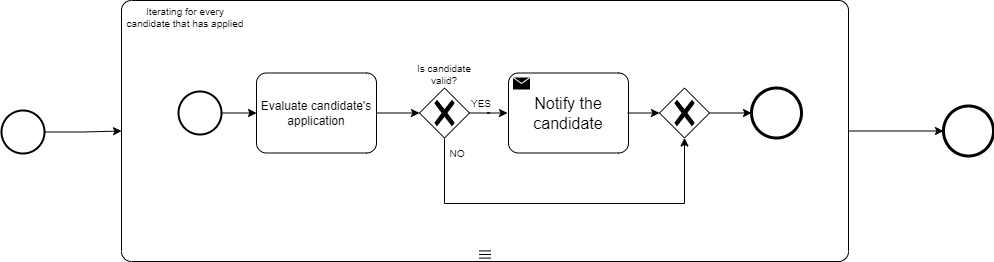
\includegraphics[scale=0.35]{images/scenario_5.png}
    \vspace{7mm}

    \item \textbf{Scenario 6: University monitors student internship progress.} \\
    Maria’s university requires students to complete an internship and uses the S\&C platform to monitor student progress. Once Maria secures the internship at CodeWorks, her university’s coordinator views her status, including the start date, role, and completion date. A dashboard allows the coordinator to track Maria’s feedback and address any concerns. If Maria or CodeWorks reports issues, the coordinator is notified, enabling them to assist in resolving challenges like scheduling conflicts or misaligned expectations.

    \item \textbf{Scenario 7: Student submits feedback and receives certificate upon internship completion.}  \\
    After completing her internship, Maria is prompted to submit feedback on her experience at CodeWorks. She completes a form rating aspects such as mentorship, skill development, and overall satisfaction. The feedback is anonymized and shared with CodeWorks for future improvement. Upon submission, the platform generates an internship completion certificate for Maria, which she can download from her profile. This certificate and feedback contribute to analyses that enhance future recommendations for students.
\end{itemize}

\newpage

\subsection{Product Functions}

The Students\&Companies (S\&C) platform serves as an intermediary between students seeking internship opportunities and companies offering them. The primary goal of the platform is to facilitate a streamlined and efficient matchmaking process, providing both students and companies with a robust set of functionalities tailored to their unique needs. Below, the most important requirements of the system are outlined, focusing on core functions that enable users to interact, apply, and manage internships effectively.

\subsubsection{G1: Student Registration and Profile Management}
    \begin{itemize}
        \item R1: Dashboard with recommended internships — The system shall provide students with a personalized dashboard displaying internships tailored to their profile, along with application statuses and feedback.
        \item R2: Profile creation and editing — Students must be able to create a profile by entering key details such as education, skills, and career interests, and be allowed to update this information to refine recommendations.
        \item R13: Detailed profile management with CV upload — The platform shall support a detailed profile structure where students can upload and manage their CV to showcase their qualifications to potential employers.
    \end{itemize}

\subsubsection{G2: Company Registration and Internship Posting}
    \begin{itemize}
        \item R5: Internship posting management — The system shall allow companies to create, update, and manage internship listings with details such as job title, required skills, duration, and benefits.
        \item R6: Company dashboard for reviewing applications — Companies should have a dashboard where they can view applications, assess candidate profiles, and filter applicants based on skills and qualifications.
        \item R14: Set deadlines and manage postings — Companies must be able to set deadlines for applications and update or close postings as positions are filled or requirements change.
    \end{itemize}

\subsubsection{G3: Suggest Suitable Internships to Students}
    \begin{itemize}
        \item R6: Recommendations based on profile match — The recommendation engine should analyze student profiles and match them with internships based on skills, interests, and career goals.
        \item R15: Machine learning for matching students and internships — The system shall use a machine learning algorithm to improve matching accuracy between students and internships over time.
        \item R16: Recommendation engine improvement based on feedback — Feedback from completed internships should feed back into the recommendation engine to enhance its accuracy for future recommendations.
    \end{itemize}

\subsubsection{G4: Suggest Suitable Students to Companies}
    \begin{itemize}
        \item R7: Recommendation feed for companies — The system shall provide companies with a list of recommended candidates whose profiles match the requirements of their internship postings.
        \item R17: Management of candidate reviews and interview feedback — Companies should be able to review applicants, manage interview feedback, and assess candidates’ fit based on their profiles and feedback received.
    \end{itemize}

\subsubsection{G5: Application Management}
    \begin{itemize}
        \item R8: Application submission directly from profile — Students should be able to apply to internships directly from their profiles by submitting their CVs and required documentation within the platform.
        \item R63: Real-time tracking of application status — The platform should provide students with real-time updates on their application status, indicating stages like "received," "under review," or "interview scheduled."
    \end{itemize}

\subsubsection{G6: Interview Management}
    \begin{itemize}
        \item R9: Application tracking for students — Students should be able to monitor their application progress, including interview scheduling and final decisions.
        \item R10: Company interview scheduling and rescheduling — Companies must be able to schedule interviews with applicants, notifying candidates and handling any rescheduling requests through the platform.
    \end{itemize}
    
\subsubsection{G7: Feedback Management}
    \begin{itemize}
        \item R11: Feedback collection and sharing for continuous improvement — After internships, the system shall collect structured feedback from both students and companies, focusing on skill relevance, job experience, and satisfaction.
        \item R18: Mutual feedback between students and companies post-internship — Both students and companies must be able to rate each other’s performance and provide feedback, contributing to an improved internship process and matching accuracy.
    \end{itemize}

    \begin{itemize}
        \item R8: University dashboard for tracking progress — Universities shall have access to a dashboard to monitor their students' internship statuses, helping support students in meeting academic and career goals.
        \item R19: Complaint management system for universities — Universities can use a complaint management system to address and resolve any reported issues between students and companies.
        \item R59: Real-time internship analytics — Universities should have access to analytics that summarize internship data, such as completion rates and popular industries, supporting curriculum and career service improvements.
    \end{itemize}




\subsection{User Characteristics}

The Students\&Companies (S\&C) platform is designed to cater to three primary types of users: students, companies, and university administrators. Each user group has unique needs and characteristics, which the platform addresses to ensure a user-friendly and effective experience. Understanding these user characteristics is essential for aligning the platform’s functionalities with user expectations and optimizing their interactions.

\subsubsection{Students}
Students are the primary user group for the S\&C platform. Generally, they are undergraduate or graduate students from diverse academic backgrounds, including engineering, business, arts, and sciences. Students are often in search of practical experience, skill development, and improved employability, making internships highly valuable for their career growth. \\ \\
The platform supports students by providing access to internship opportunities that match their specific skills, academic background, and career aspirations. With a simplified application process, students can easily apply for internships and submit their CVs directly through the platform, making the process efficient and accessible. To enhance the likelihood of securing a position, students receive regular notifications about new and recommended internships aligned with their profile, ensuring they don’t miss out on opportunities. Additionally, students can track the status of their applications, allowing them to stay informed about each step of the process. To further support career development, the S\&C platform offers students guidance on improving their CVs and profiles, enhancing their chances of selection for internships.

\subsubsection{Companies}
Companies on the S\&C platform range from small startups to large enterprises across various industries, each seeking talented interns who can support their teams, bring fresh perspectives, and contribute to ongoing projects. Depending on the company size, internship management may fall under HR personnel or directly with team managers. \\ \\
For companies, the S\&C platform offers a straightforward registration process and an intuitive interface to post internships, allowing them to quickly reach a large pool of qualified students. Companies benefit from easy access to student profiles and CVs, enabling them to identify candidates with the skills and experiences that best fit their requirements. The platform also provides tools to manage applications efficiently, from the review stage through to scheduling interviews and interacting with students directly. After internships conclude, companies can leave feedback to improve future offerings and to enhance the platform’s recommendation algorithms. Overall, the S\&C platform provides a centralized system for companies to post, manage, and evaluate internship candidates with ease and effectiveness.

\subsubsection{University Administrators}
University administrators, particularly those involved in career services or specific academic departments, use the platform to oversee their students’ internship experiences and ensure they align with academic requirements. This group may include career service coordinators, faculty advisors, and program managers who play an active role in supporting students during their internships.\\ \\
For universities, the S\&C platform includes a monitoring dashboard that allows administrators to track students’ internship statuses, review student feedback, and provide support when necessary. This feature is essential for maintaining an overview of students’ progress and ensuring that internships meet academic standards. Additionally, administrators can mediate any complaints or issues that arise between students and companies, facilitating resolution and safeguarding the quality of the internship experience. Access to reports and aggregated data on student internship outcomes also enables universities to assess and refine their internship programs, enhancing the overall educational value of these experiences.
\\ \\
By tailoring specific features to address the characteristics of students, companies, and university administrators, the S\&C platform provides a well-rounded and effective solution. Each user group’s needs are met through targeted functionalities, creating a cohesive and supportive environment for successful internship placements and professional development.



\subsection{Assumptions, Dependencies, and Constraints}
\begin{itemize}
    \item \textbf{Internet Availability}: The platform assumes users have access to a stable internet connection to interact with the web-based interface.
    \item \textbf{Data Privacy}: The platform must comply with GDPR regulations, ensuring that all personal data from students and companies is handled securely and transparently.
    \item \textbf{Scalability}: The system must be able to scale to accommodate multiple universities and thousands of users simultaneously.
    \item \textbf{Cross-browser Compatibility}: The platform should work on all major browsers (e.g., Chrome, Firefox, Safari) and on both desktop and mobile devices.
    \item \textbf{Interoperability}: The platform must be able to integrate with university systems for student verification and internship tracking.
\end{itemize}

\subsection{Domain Assumptions}

\begin{longtable}{|p{1cm}| p{4cm} | p{5cm} |}
\hline
\textbf{ID} & \textbf{Assumption} & \textbf{Description} \\ 
\hline
\textbf{DA1} & Students need internships to gain practical experience & 
University students actively seek internships as part of their professional development. \\ 
\hline
\textbf{DA2} & Companies need interns for various projects & 
Companies value interns and use internships as a talent pool to find potential full-time employees. \\ 
\hline
\textbf{DA3} & Students have varied skills and interests & 
Students have different qualifications, skills, and career aspirations that may influence their internship search. \\ 
\hline
\textbf{DA4} & Companies have specific internship requirements & 
Companies offer internships with specific requirements, such as particular skills, qualifications, or experiences. \\ 
\hline
\textbf{DA5} & Keyword and recommendation-based searches are helpful & 
Searching by keywords and personalized recommendation algorithms can improve internship matches. \\ 
\hline
\textbf{DA6} & Communication between students, companies, and universities is crucial & 
There is a need for communication and feedback loops among all parties involved in internships. \\ 
\hline
\textbf{DA7} & Both parties (students and companies) need tools for managing applications, interviews, and assessments & 
Interviews and assessments are a crucial part of the selection process, and digital tools will help facilitate this process. \\ 
\hline
\textbf{DA8} & Universities are interested in monitoring internship quality & 
Universities play a role in ensuring the quality of internships and supporting students and companies where necessary. \\ 
\hline
\end{longtable}

\newpage
